% This is samplepaper.tex, a sample chapter demonstrating the
% LLNCS macro package for Springer Computer Science proceedings;
% Version 2.20 of 2017/10/04
%
\documentclass[runningheads]{llncs}
%
\usepackage{verbatim}
\usepackage{graphicx}
% Used for displaying a sample figure. If possible, figure files should
% be included in EPS format.
%
% If you use the hyperref package, please uncomment the following line
% to display URLs in blue roman font according to Springer's eBook style:
% \renewcommand\UrlFont{\color{blue}\rmfamily}

\begin{document}
%
\title{Modality Independence for Parameterized Mood Expression in Humanoids}
%
%\titlerunning{Abbreviated paper title}
% If the paper title is too long for the running head, you can set
% an abbreviated paper title here
%
\author{Apoorva Arora\inst{1} \and
Aishwarya Shastry\inst{2} \and
Gautam Miglani\inst{3}}
%
\authorrunning{A Arora et al.}
% First names are abbreviated in the running head.
% If there are more than two authors, 'et al.' is used.
%
\institute{Delft University of Technology Intelligent Systems Department
The Netherlands
\email{\{A.Arora-1,A.shastry,G.Miglani\}@student.tudelft.nl}}
%
\maketitle              % typeset the header of the contribution
%
\begin{abstract}

\keywords{Robot Mood\and  \and Another keyword.}
\end{abstract}
%
%
%
\section{Introduction}
Study in the field of Emotion expression in robots and virtual agents is becoming increasingly popular. The goal being able to find if it is possible for robots to portray emotions in the same manner as humans.Expression of mood, beliefs and intentions by robots is important to improve their life-like quality in Human Robot Interactions\cite{1}. The research in the area of continuous expression of emotional state by a robot while it is involved in its intended task is relatively novel.

\begin{comment}
Here you present the actual review of your target paper’s topic. Don’t attack it, review the topic and the findings in the paper critically on their up- and downsides. Also include related work that you need in order to have the reader understand your review and point of view. This is in fact the typical “motivation and related work” section in a paper as this section should critically describe the work of others and how those works relate to your project. Issues to be covered include all stuff related to eventually understanding why you propose the question you want to address in section 2.
\end{comment}

\subsection{Motivation and related work}
The aim of our study is to integrate bodily and speech expression of mood with functional behaviour(task execution) of a robot. Different 'styles' or 'quality' of execution of a functional behaviour reflect emotions and help humans to understand the mood of robots.\cite{joost}. In our study, we focus on the expression of mood by modulation of the 'style' of speech (talking) and bodily movements such as walking, hand movements and standing posture.'Style' is characterized by  parameters of behaviour such as speed, intensity, extent and regularity.\cite{angelica}.\\ Xu et al\cite{joost} in their paper \textit{Bodily Mood Expression: Recognize Moods from Functional Behaviors of Humanoid Robots} used Amplitude, Repetition, Hold Time, Decay Speed as some of the behaviour parameters. They used two behaviours waving and finger pointing and applied behaviour parameter modulation under three conditions:
\begin{enumerate}
    \item Modulating all parameters
    \item Modulating only important parameters
    \item Modulating only unimportant parameters
\end{enumerate}
They obtained behaviour parameter settings from a design experiment corresponding to different moods. They then evaluated these settings using a recognition experiment to find out of if people are able to recognize the mood from the modulated functional behaviour of humanoid NAO.
They studied emotions in two dimensions-Valence and Arousal(The Valence Arousal model\cite{valence}).Their study found that modulation of All parameters and Important parameters enabled people to successfully recognize the mood of NAO. While, modulation of unimportant parameters could only express weak mood.
The primary goal of our study is to establish that modulation of the behaviour parameters translates uniformly across different modalities of emotion expression, in our case speech and bodily movements. For instance, increasing speed of speech and hand movements both must indicate anger. Further, we investigate that which parameters exhibit this uniformity to discover common features across modalities. For our study, we use the term emotion and mood interchangeably, since the two terms are strongly related. Ekman\cite{ekman} in his work on universal facial expressions lists 6 emotions: fear, anger,sadness, happiness, disgust and surprise. Tomkins \cite{tomkins} includes interest and shame;Johnson-Laird and Oatley list 5 emotions: fear, anger, sadness, happiness and disgust\cite{oatley}. Thus, the most common four emotions are fear, anger, sadness and joy\cite{angelica}. These four emotions form the basis of our study.Further,similar to  Xu et al\cite{joost}  we use Russell’s circumplex model of affect \cite{russell}, which represents emotion along two axes: arousal and valence. We will be using NAO for our experiment\cite{nao} because of its feasibility, user friendly interface and support for different programming languages.
\begin{figure}
\centering
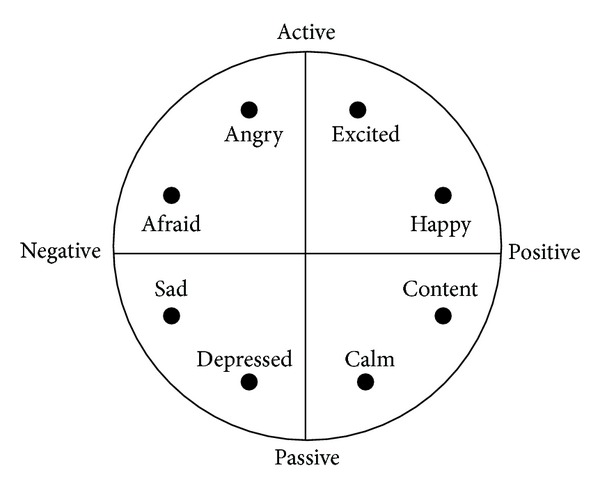
\includegraphics[width = 3in]{valence.png}
\caption{Valence Arousal Model}
\label{valence}
\end{figure}

%parameters

\\
%write about NAOMOR
%intro
%critic
Xu et al \cite{joost} in their work obtain a relation between behaviour parameters  and valence for each behaviour through a design task. It is not clear how they established a test relation between arousal and parameters. In addition, arousal was not considered while defining important parameters.Also, the implementation of the design experiment is unclear.Besides,they used 26 subjects for the experiment where half of them belonged to the same nationality. It is important to use a diverse set of subjects to reach at unbiased results. Further,employing parameter modulation of a wide range of behaviours involving different modalities, would enable more concrete and consistent results.
%They obtain important parameters from the task which asks participants to design mood expression  according to valence and ignore arousal and consider two modalities- waving and pointing for the experiment.  We plan to use paired comparison to test perceived valence and arousal among people as mentioned in the paper as it gives more precise results in interval scales. The experiment considers 26 participants, half of them being Chinese. This might result in inconsistencies while detecting emotion. We propose to test a more diverse set of people with different nationalities.


\section{Research question}
Junchao Xu et al \cite{joost} used two behaviours from a single modality to successfully show that robots are capable of expressing moods through modulated functional behaviour. We propose to use the parameterized functional behaviour model to establish that a given parameter setting express same mood in different modalities. Further, investigate which parameters behave uniformly across modalities. The result of our study would allow synthesis of emotions/mood in different modalities using a standard and unifying model. For example, the model will allow learning mood characteristics from speech and apply to posture/movements. Thus, we arrive at following research questions:
\begin{enumerate}
    \item How modulation of various behavior parameters influence the expression of emotions/mood across modalities? That is, Is behaviour parameters modulation independent of the modality of emotion/mood expression?
 \item Which behaviour parameters are uniform across two modalities and what are the common features of the modalities?
\end{enumerate}
\subsection{Hypotheses}
\begin{enumerate}
\item Behaviour parameters modulation is independent of the modality of emotion/mood expression.
\item Exhibition of mood through different modalities have same underlying behaviour (eg. intensity, speed, regularity etc.)
\item A given behaviour parameter setting reflects the same emotion/mood in speech and body movement modalities.

%A hypothesis is a testable yes/no question derived from your research question. For example: nice weather increases the number of incidents on highways.
\end{enumerate}
\section{Method}
This Experiment would be carried out in four steps:
\begin{enumerate}
   % \item Questionnaire to find out potential parameters for the experiment  
    \item Finding out potential parameters and their relation with valence and arousal for speech and bodily movement modalities using existing Literature Study.
    \item Designing the experiment(programming NAO) using results from step 1.
    \item User Study to evaluate the recognition of Robot's mood in different modalities.
    \item Carry Statistical Analysis to answer proposed research questions.
\end{enumerate}

\begin{comment}
You describe how you study your hypotheses, what kind of approach you took (e.g., an experiment). If you write the proposal, you will have to write section 3.4, in the final paper that is left out.
\end{comment}
\subsection{Materials}
To develop our system , we first need to find out the parameters which would be important to describe an emotion via the two modalities.
To find the important parameters we plan to read research papers in this domain and come up with some potential parameters for modelling.

\begin{comment}
You describe the material you used (i.e., the system you developed, the experimental materials used to test the system)
\end{comment}


\subsection{Experimental setup / approach}
% dataset should be diverse with people of different sex, nationality and age group 18-30
%You describe how the experiment was setup (is applicable).
After finding parameters and coding them in NAO, we would like to test if people can recognize the mood via different modalities. We plan to test the model on a set of participants from Delft University of Technology with ages 18-35 and different place of origin(Nationalities). We use a 0-9 scale of Valence and Arousal to label the moods depicted by the robot. For that, we explain the participants about Valence Arousal Model. We use various parameters settings corresponding to different moods and apply each setting to both the body modality and speech modality. Participants are asked to give a no. to the expressed mood on the valence-arousal scale and what mood is the robot expressing. Finally they are asked which parameter depicts their selected mood the most.

\subsection{ Measures}
To answer our proposed research questions we would like to measure uniformity of these parameters for various emotions in different modalities. For this purpose, we calculate correlation between different modalities for a specific parameter reflecting a specific mood.For instance, calculating the correlation between modality speech and body for parameter high speed.The correlation factor reflects the probability that high speed would relate to high valence in both the modalities.
%We can use Pearson Correlation for this  experiment.
%You probably have to measure something in order to test you hypothesis. This is where you explain what and how you measure this. For example, nice weather is measured as the average temperature over the day and incidents are all by the police reported traffic incidents on registered highways.

\subsection{Work plan}
\begin{enumerate}
\item Week 0- Project Selection and Proposal
    \item Week 1- Decide the parameters for the experiment by reading papers in the domain.
    \item Week 2- Carrying out the Experiment with NAO 
    \item Week 3- Carrying out the Experiment with NAO
    \item Week 4- Mid term Presentation and Evaluation form Subjects
    \item Week 5- Drawing conclusions and working for Final Presentation and Paper
   \item Week 6- Final Presentation and Paper submission 
\end{enumerate}
\section{Results}



\subsection{ Discussion}




\begin{comment}
\subsubsection{Sample Heading (Third Level)} Only two levels of
headings should be numbered. Lower level headings remain unnumbered;
they are formatted as run-in headings.

\paragraph{Sample Heading (Fourth Level)}
The contribution should contain no more than four levels of
headings. Table~\ref{tab1} gives a summary of all heading levels.
%%
\begin{table}
\caption{Table captions should be placed above the
tables.}\label{tab1}
\begin{tabular}{|l|l|l|}
\hline
Heading level &  Example & Font size and style\\
\hline
Title (centered) &  {\Large\bfseries Lecture Notes} & 14 point, bold\\
1st-level heading &  {\large\bfseries 1 Introduction} & 12 point, bold\\
2nd-level heading & {\bfseries 2.1 Printing Area} & 10 point, bold\\
3rd-level heading & {\bfseries Run-in Heading in Bold.} Text follows & 10 point, bold\\
4th-level heading & {\itshape Lowest Level Heading.} Text follows & 10 point, italic\\
\hline
\end{tabular}
\end{table}


\noindent Displayed equations are centered and set on a separate
line.
\begin{equation}
x + y = z
\end{equation}
Please try to avoid rasterized images for line-art diagrams and
schemas. Whenever possible, use vector graphics instead (see
Fig.~\ref{fig1}).

\begin{figure}
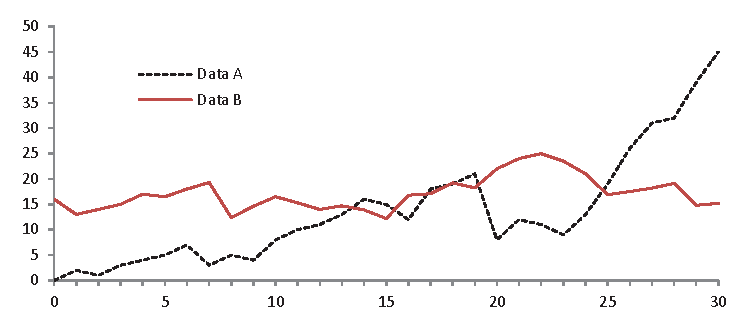
\includegraphics[width=\textwidth]{fig1.eps}
\caption{A figure caption is always placed below the illustration.
Please note that short captions are centered, while long ones are
justified by the macro package automatically.} \label{fig1}
\end{figure}

\begin{theorem}
This is a sample theorem. The run-in heading is set in bold, while
the following text appears in italics. Definitions, lemmas,
propositions, and corollaries are styled the same way.
\end{theorem}
%
% the environments 'definition', 'lemma', 'proposition', 'corollary',
% 'remark', and 'example' are defined in the LLNCS documentclass as well.
%
\begin{proof}
Proofs, examples, and remarks have the initial word in italics,
while the following text appears in normal font.
\end{proof}
\end{comment}
\section{Conclusion and further research}
%
% ---- Bibliography ----
%
% BibTeX users should specify bibliography style 'splncs04'.
% References will then be sorted and formatted in the correct style.
%
% \bibliographystyle{splncs04}
% \bibliography{mybibliography}
%
\begin{thebibliography}{8}
\bibitem{1}
Breazeal, C., Takanishi, A., Kobayashi, T.: Social robots that interact with people. Springer Handbook of Robotics, pp. 1349-1369. Springer, Berlin, (2008)
\bibitem{joost}
Xu J., Broekens J., Hindriks K., Neerincx M.A. (2013) Bodily Mood Expression: Recognize Moods from Functional Behaviors of Humanoid Robots. In: Herrmann G., Pearson M.J., Lenz A., Bremner P., Spiers A., Leonards U. (eds) Social Robotics. ICSR 2013. Lecture Notes in Computer Science, vol 8239. Springer, Cham 
\bibitem{angelica}
Angelica LIM, Design and Implementation of Emotions for Humanoid Robots based on the Modality-independent DESIRE Model, Master Thesis
\bibitem{nao}
Shamsuddin, S., Ismail, L. I., Yussof, H., Zahari, N. I., Bahari, S., Hashim, H., and Jaffar, A. (2011). Humanoid robot NAO: Review of control and motion exploration. In Proceedings - 2011 IEEE International Conference on Control System, Computing and Engineering, ICCSCE 2011 (pp. 511-516). [6190579] DOI: 10.1109/ICCSCE.2011.6190579
\bibitem{valence}
Grekow J. (2018) Representations of Emotions. In: From Content-based Music Emotion Recognition to Emotion Maps of Musical Pieces. Studies in Computational Intelligence, vol 747. Springer, Cham
\bibitem{ekman}
Ekman, P. (2005). Basic Emotions. In Handbook of Cognition and Emotion (eds T. Dalgleish and M. J. Power). doi:10.1002/0470013494.ch3
\bibitem{tomkins}
SS Tomkins, Affect theory. In KR Scherer and P Ekman (Eds.), Approaches to
emotion, pp. 163-195. Hillsdale, NJ: Erlbaum (1984)
\bibitem{oatley}K Oatley and PN Johnson-Laird, Towards a cognitive theory of emotions. Cognition and Emotion, 1, 29-50 (1987)
\bibitem{russell}
Russell, J. A. (1980). A circumplex model of affect. Journal of Personality and Social Psychology, 39(6), 1161-1178. http://dx.doi.org/10.1037/h0077714
\begin{comment}


\bibitem{ref_lncs1}
Author, F., Author, S.: Title of a proceedings paper. In: Editor,
F., Editor, S. (eds.) CONFERENCE 2016, LNCS, vol. 9999, pp. 1--13.
Springer, Heidelberg (2016). \doi{10.10007/1234567890}

\bibitem{ref_book1}
Author, F., Author, S., Author, T.: Book title. 2nd edn. Publisher,
Location (1999)

\bibitem{ref_proc1}
Author, A.-B.: Contribution title. In: 9th International Proceedings
on Proceedings, pp. 1--2. Publisher, Location (2010)

\bibitem{ref_url1}
LNCS Homepage, \url{http://www.springer.com/lncs}. Last accessed 4
Oct 2017
\end{comment}
\end{thebibliography}
\end{document}
